\chapter{Arhitektura i dizajn sustava}

		{ Arhitektura sustava je hijerarhijska, dakle svaki pojedini sloj
			komunicira isključivo sa slojevima koji su neposredno ispred i iza njega. Slojevi sustava koje mi implementiramo jesu:}
	\begin{itemize}
		\item 	\textit{Korisničko sučelje}
		\item 	\textit{Kontroler}
		\item 	\textit{Servis}
		\item 	\textit{Repozitorij}
		\item 	\textit{Baza podataka}
	\end{itemize}

		{Korisničko sučelje (eng. User interface, UI) predstavlja interaktivno područje između korisnika i računala. Njegov je glavni cilj omogućiti korisnicima učinkovito korištenje i upravljanje računalom te osigurati da računalo pruži korisniku potrebne informacije.\\

			Za izradu korisničkog sučelja u ovom slučaju korišten je React, JavaScript biblioteka koja omogućava brzo i jednostavno stvaranje interaktivnih korisničkih sučelja. Kroz korisničko sučelje, korisnik šalje zahtjeve kontroleru, a kontroler potrebne podatke prosljeđuje pomoću JSON (JavaScript Object Notation) datoteka.\\

			JSON datoteke služe za pohranu i prijenos podataka u obliku ključ-vrijednost. Nakon što korisničko sučelje preda JSON datoteku, ono očekuje odgovor od kontrolera koji će također biti u JSON formatu. Kontroler u ovom slučaju predstavlja REST API (representational state transfer) te obrađuje zahtjeve vanjskih potrošača.\\

			Servis je odgovoran za obradu podataka koje prima od korisničkog sučelja putem kontrolera i baze podataka putem repozitorija. Osim toga, servis obuhvaća poslovne odluke, autorizaciju te provjeru valjanosti identiteta korisnika.\\

			Repozitorij ima ulogu komunikacije s bazom podataka te uključuje funkcije za pronalaženje određenih objekata ili skupina objekata iz baze podataka. Ove funkcije obično vraćaju popis objekata koji zadovoljavaju određeni uvjet.\\

			Baza podataka koristi se za pohranu i upravljanje podacima te predstavlja ključni dio sustava koji omogućuje trajno čuvanje informacija.\\

			Kontroler, servis i repozitorij implementirani su pomoću Java Spring Boota, te su pisani u jeziku JavaScript.}


		\section{Baza podataka}

		Za potrebe sustava koji implementiramo koristit ćemo se relacijskom bazom podataka koja kao svoju glavnu namjenu ima olakšano modeliranje stvarnog svijeta oko nas. Gradivna jedinica baze jest relacija (tablica) koja je definirana svojim imenom te skupom atributa. Baza podataka ove aplikacije sastoji se od sljedećih entiteta:
		\begin{itemize}
		\item 	\textit{Konferencija}
		\item 	\textit{Korisnik}
		\item 	\textit{Poster}
		\item 	\textit{FotoMaterijal}
		\item 	\textit{PromoMaterijal}
	\end{itemize}

			\subsection{Opis tablica}


				{Konferencija - centralni entitet koji definira događaj kojemu pristupaju sudionici, bilo autori ili ne. Atributi koje posjeduje su \textit{konfID}, \textit{kod} (za pristup posterima koji su u natjecanju), \textit{datPocetak}, \textit{datKraj}, \textit{nazivKonf}, \textit{mjestoKonf}, \textit{opisKonf}}


				\begin{longtblr}[
					label=none,
					entry=none
					]{
						width = \textwidth,
						colspec={|X[6,l]|X[10, l]|X[20, l]|},
						rowhead = 1,
					} %definicija širine tablice, širine stupaca, poravnanje i broja redaka naslova tablice
					\hline \SetCell[c=3]{c}{\textbf{Konferencija}}	 \\ \hline[3pt]
					\SetCell{LightGreen}konfID & INT	&  	Jedinstveni identifikator konferencije  	\\ \hline
					kod	& INT & Pristupna lozinka za posjetitelje  	\\ \hline
					vrijemePoc & LOCALDATETIME & Vrijeme početka konferencije \\ \hline
					vrijemeKraj & LOCALDATETIME	& Vrijeme kraja konferencije 		\\ \hline
					nazivKonf & VARCHAR	& Naziv konferencije 		\\ \hline
					opisKonf & VARCHAR	& Opis konferencije 		\\ \hline
					\SetCell{LightBlue} pbr	& INT &   	Poštanski broj mjesta održavanja konferencije\\ \hline
				\end{longtblr}

				{Mjesto - entitet koji definira mjesto u kojemu se održava konferencija. Atributi koje posjeduje su \textit{kucBroj} i \textit{ulica} kao glavni ključ, \textit{nazivMjesta} i \textit{pbr}.  Mjesto je u vezi jedan-prema-više s entitetom Konferencija. Odnosno jedna konferencija ima jedno mjesto, dok jedno mjesto ima više konferencija.}


				\begin{longtblr}[
					label=none,
					entry=none
					]{
						width = \textwidth,
						colspec={|X[6,l]|X[6, l]|X[20, l]|},
						rowhead = 1,
					} %definicija širine tablice, širine stupaca, poravnanje i broja redaka naslova tablice
					\hline \SetCell[c=3]{c}{\textbf{Mjesto}}	 \\ \hline[3pt]
					\SetCell{LightGreen}kucBroj & INT	&  	Kućanski broj ulice u kojoj će se održavati konferencija\\ \hline
					\SetCell{LightGreen}ulica & VARCHAR	&  	Ulica u kojoj će se održavati konferencija  	\\ \hline
					nazivMjesta	& VARCHAR & Naziv mjesta gdje se održava konferencija  	\\ \hline
					pbr & INT	& Poštanski broj mjesta održavanja konferencije  		\\ \hline
				\end{longtblr}




				{FotoMaterijal - entitet FotoMaterijal koristi nam kako bismo mogli pohraniti fotografije nastale tijekom konferencije te ih kasnije prikazati korisnicima. Sadrži atribute: \textit{fotoID}, \textit{nazivFoto}, \textit{fotoPath} te strani ključ \textit{konfID} pomoću kojega možemo upariti kojoj konferenciji pripada koja fotografija (veza jedan-prema-više).}


				\begin{longtblr}[
					label=none,
					entry=none
					]{
						width = \textwidth,
						colspec={|X[6,l]|X[6, l]|X[20, l]|},
						rowhead = 1,
					}
					\hline \SetCell[c=3]{c}{\textbf{FotoMaterijal}}	 \\ \hline[3pt]
					\SetCell{LightGreen}fotoID & INT	&  Jedinstveni identifikator fotografije	\\ \hline
					nazivFoto	& VARCHAR &   Naziv fotografije\\ \hline
					fotoPath & VARCHAR &   Putanja do izvora fotografije\\ \hline
					\SetCell{LightBlue} konfID	& INT &   	Jedinstveni identifikator konferencije\\ \hline
				\end{longtblr}


				{Korisnik - entitet kojim se pokriva registrirani korisnik, neregistrirani korisnik te autor. Sadrži atribute \textit{email} te \textit{lozinka} kojima se kasnije može pristupiti posebnom sadržaju specifičnom za registrirane korisnike. Također sadrži \textit{ime} i \textit{prezime} i \textit{ulogaID} koji je strani ključ preko kojeg je entitet Korisnik spojen vezom više-prema-više s entitetom Uloge.}


				\begin{longtblr}[
					label=none,
					entry=none
					]{
						width = \textwidth,
						colspec={|X[6,l]|X[6, l]|X[20, l]|},
						rowhead = 1,
					} %definicija širine tablice, širine stupaca, poravnanje i broja redaka naslova tablice
					\hline \SetCell[c=3]{c}{\textbf{Korisnik}}	 \\ \hline[3pt]
					\SetCell{LightGreen}email & VARCHAR	&  Elektronička pošta korisnika	\\ \hline
					lozinka	& VARCHAR &  Lozinka za prijavu korisnika	\\ \hline
					ime	& VARCHAR &  Ime korisnika	\\ \hline
					prezime	& VARCHAR &  Prezime korisnika	\\ \hline
					\SetCell{LightBlue} ulogaID	& INT &   	Jedinstveni identifikator uloge\\ \hline
				\end{longtblr}

				{Uloge - entitet kojim se pokrivaju koje uloge sve postoje kao i koje uloge imaju korisnici. Atributi koje sadrži entitet Uloge su: \textit{ulogaID} koji je glavni ključ i \textit{uloga} koja opisuje o kojoj je ulozi riječ.}


				\begin{longtblr}[
					label=none,
					entry=none
					]{
						width = \textwidth,
						colspec={|X[6,l]|X[6, l]|X[20, l]|},
						rowhead = 1,
					} %definicija širine tablice, širine stupaca, poravnanje i broja redaka naslova tablice
					\hline \SetCell[c=3]{c}{\textbf{Uloge}}	 \\ \hline[3pt]
					\SetCell{LightGreen}ulogaID & ID	&  Jedinstveni identifikator uloge	\\ \hline
					uloga	& VARCHAR &  Uloga korisnika	\\ \hline
				\end{longtblr}

				{Poster - ovim entitetom kontrolirat će se radovi koje na konferenciju dostavljaju autori te se na njoj izlažu i za njih se može glasati. Njegovi atributi su: \textit{posterID}, \textit{nazivPoster}, \textit{posterPath}, \textit{email}, \textit{imeAutor}, \textit{prezimeAutor}, \textit{brojGlasova} i \textit{konfID} koji je ujedno i strani ključ pomoću kojega možemo upariti kojoj konferenciji pripada koji poster (veza jedan-prema-više).}


				\begin{longtblr}[
					label=none,
					entry=none
					]{
						width = \textwidth,
						colspec={|X[6,l]|X[6, l]|X[20, l]|},
						rowhead = 1,
					} %definicija širine tablice, širine stupaca, poravnanje i broja redaka naslova tablice
					\hline \SetCell[c=3]{c}{\textbf{Poster}}	 \\ \hline[3pt]
					\SetCell{LightGreen}posterID & INT	&  	Jedinstveni identifikator postera\\ \hline
					nazivPoster	& VARCHAR &   Naziv postera	\\ \hline
					posterPath & VARCHAR &   Putanja do izvora postera\\ \hline
					email	& VARCHAR &   Elektronička pošta korisnika\\ \hline
					imeAutor & VARCHAR &   Ime autora postera\\ \hline
					prezimeAutor & VARCHAR &   Prezime autora postera\\ \hline
					brojGlasova & INT &   Ostvareni broj glasova postera\\ \hline
					\SetCell{LightBlue} konfID	& INT &  Jedinstveni identifikator konferencije	\\ \hline
				\end{longtblr}

				{PromoMaterijal - entitet PromoMaterijal pokriva konkretan ponuđeni materijal kojemu registrirani korisnik može pristupiti. Atributi koje ima su \textit{promoId}, \textit{nazivPromo}, \textit{url}, \textit{promoPath} i \textit{konfID} koji je ujedno i strani ključ pomoću kojega možemo upariti kojoj konferenciji pripada koji promotivni materijal (veza jedan-prema-više).}


				\begin{longtblr}[
					label=none,
					entry=none
					]{
						width = \textwidth,
						colspec={|X[6,l]|X[6, l]|X[20, l]|},
						rowhead = 1,
					} %definicija širine tablice, širine stupaca, poravnanje i broja redaka naslova tablice
					\hline \SetCell[c=3]{c}{\textbf{PromoMaterijal}}	 \\ \hline[3pt]
					\SetCell{LightGreen}promoId & INT	&  Jedinstveni identifikator promotivnog materijala\\ \hline
					nazivPromo	& VARCHAR &   Naziv promotivnog materijala	\\ \hline
					promoPath & VARCHAR &  Putanja do izvora sadržaja promotivnog materijala \\ \hline
					url & VARCHAR &  WEB stranica pokrovitelja \\ \hline
					\SetCell{LightBlue} konfID	& INT &   Jedinstveni identifikator konferencije	\\ \hline
				\end{longtblr}

				{Glasanje - entitet Glasanje služi za prebrojavanje broja glasova postera te također služi za prevenciju glasovanja jednog registriranog korisnika za više postera. Atributi koji sadrži entitet Glasanje su: \textit{posterID} koji je jedinstveni identifikator postera te je također i primarni ključ, \textit{konfID} koji je jedinstveni identifikator konferencije te je također i strani ključ \textit{email} koji je elektronička pošta korisnika, ali je isto tako i strani ključ. Obje veze od entiteta Glasanje prema entitetima Korisnik i Konferencija su jedan-prema-više.}


				\begin{longtblr}[
					label=none,
					entry=none
					]{
						width = \textwidth,
						colspec={|X[6,l]|X[6, l]|X[20, l]|},
						rowhead = 1,
					} %definicija širine tablice, širine stupaca, poravnanje i broja redaka naslova tablice
					\hline \SetCell[c=3]{c}{\textbf{Glasanje}}	 \\ \hline[3pt]
					\SetCell{LightGreen}posterID & INT	&  Jedinstveni identifikator postera\\ \hline
					\SetCell{LightBlue} konfID	& INT &   Jedinstveni identifikator konferencije	\\ \hline
					\SetCell{LightBlue} email	& VARCHAR &   Elektronička pošta korisnika	\\ \hline
				\end{longtblr}



			\subsection{Dijagram baze podataka}
					\begin{figure}[H]
					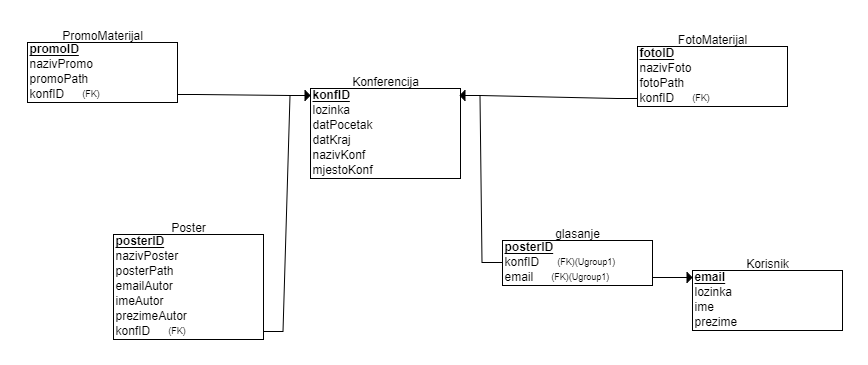
\includegraphics[width=1.2\textwidth]{slike/bazaPodataka.PNG} %veličina u odnosu na širinu linije
					\caption{Dijagram baze podataka}
					\label{fig:promjene4} %label mora biti drugaciji za svaku sliku
				\end{figure}

			\eject


		\section{Dijagram razreda}

		Zbog lakše organizacije projekta, svi kontroler razredi koji su zaduženi za upravljanje krajnijm točkama svrstani su u paket \textit{src/main/java/opp/rest}. Kontroleri igraju ključnu ulogu u upravljanju HTTP zahtjevima te su odgovorni za primanje zahtjeva od klijenta, obradu tih zahtjeva i generiranje odgovora. U našoj implementaciji imamo više kontrolera kako bi lakše organizirali i razdvojili sve dostupne krajnje točke. Npr. razred KonferencijaController zadužen je za obradu zahtjeva poput stvaranja konferencija, ulaska u konferenciju i dohvaćanja osnovnih informacija o konferenciji.

		\begin{figure}[H]
			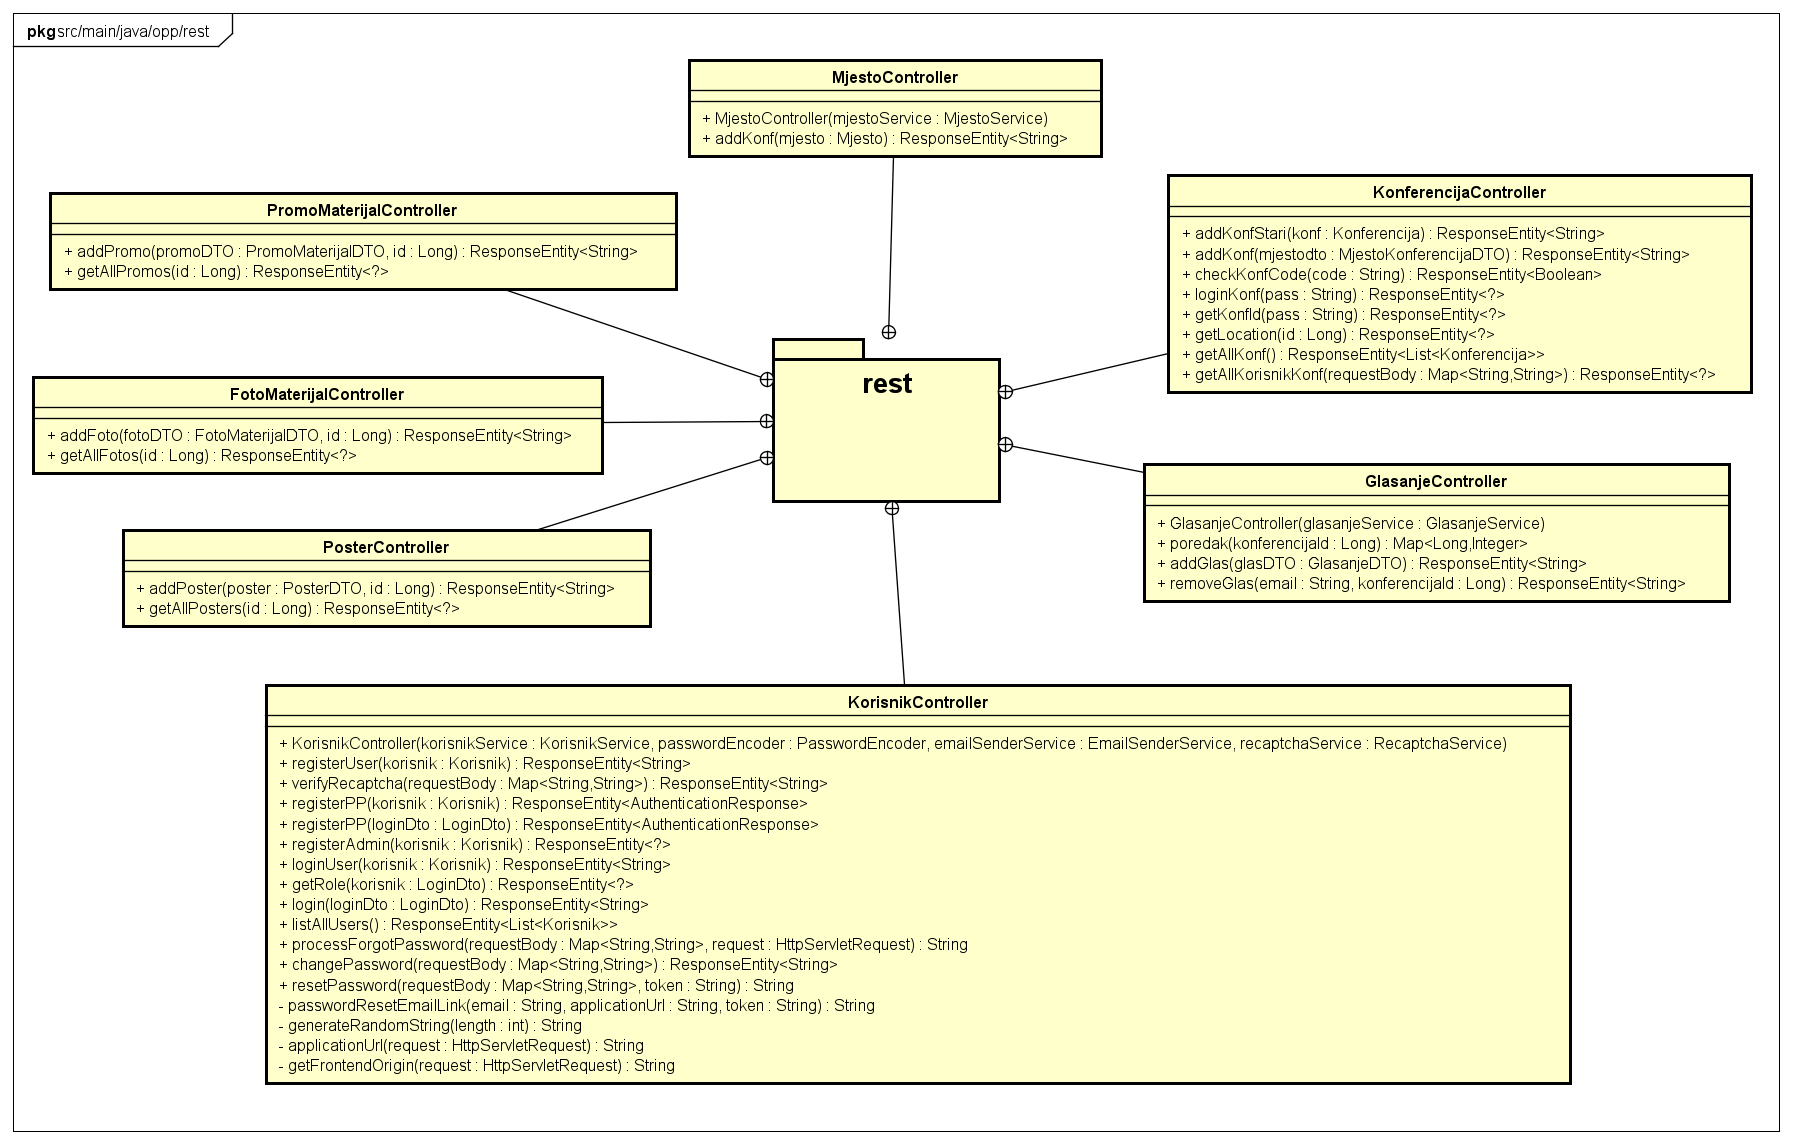
\includegraphics[width=\textwidth]{slike/controllersClassDiagram.PNG} %veličina u odnosu na širinu linije
			\caption{Dijagram razreda - Controllers}
			\label{fig:dr-controllers} %label mora biti drugaciji za svaku sliku
		\end{figure}
		\newpage
		Svi razredi zaduženi za entitete i DTO (Data Transfer Objects) smješteni su u \textit{src/main/java/opp/domain} paket. Razredi entiteta poput Konferencija, Poster, Mjesto itd. objekti su koji predstavljaju podatke u bazi podataka te su odgovorni za mapiranje objekata u redove u tablici baze podataka i obrnuto. Također, sadrže načine upravljanja podatcima i njihovu validaciju (osiguravaju integritet baze podataka). Razredi DTO također su objekti koji se koriste za razmjenu podataka između aplikacija, a u našem je slučaju to komunikacija između backend i frontend dijela.
		\begin{figure}[H]
			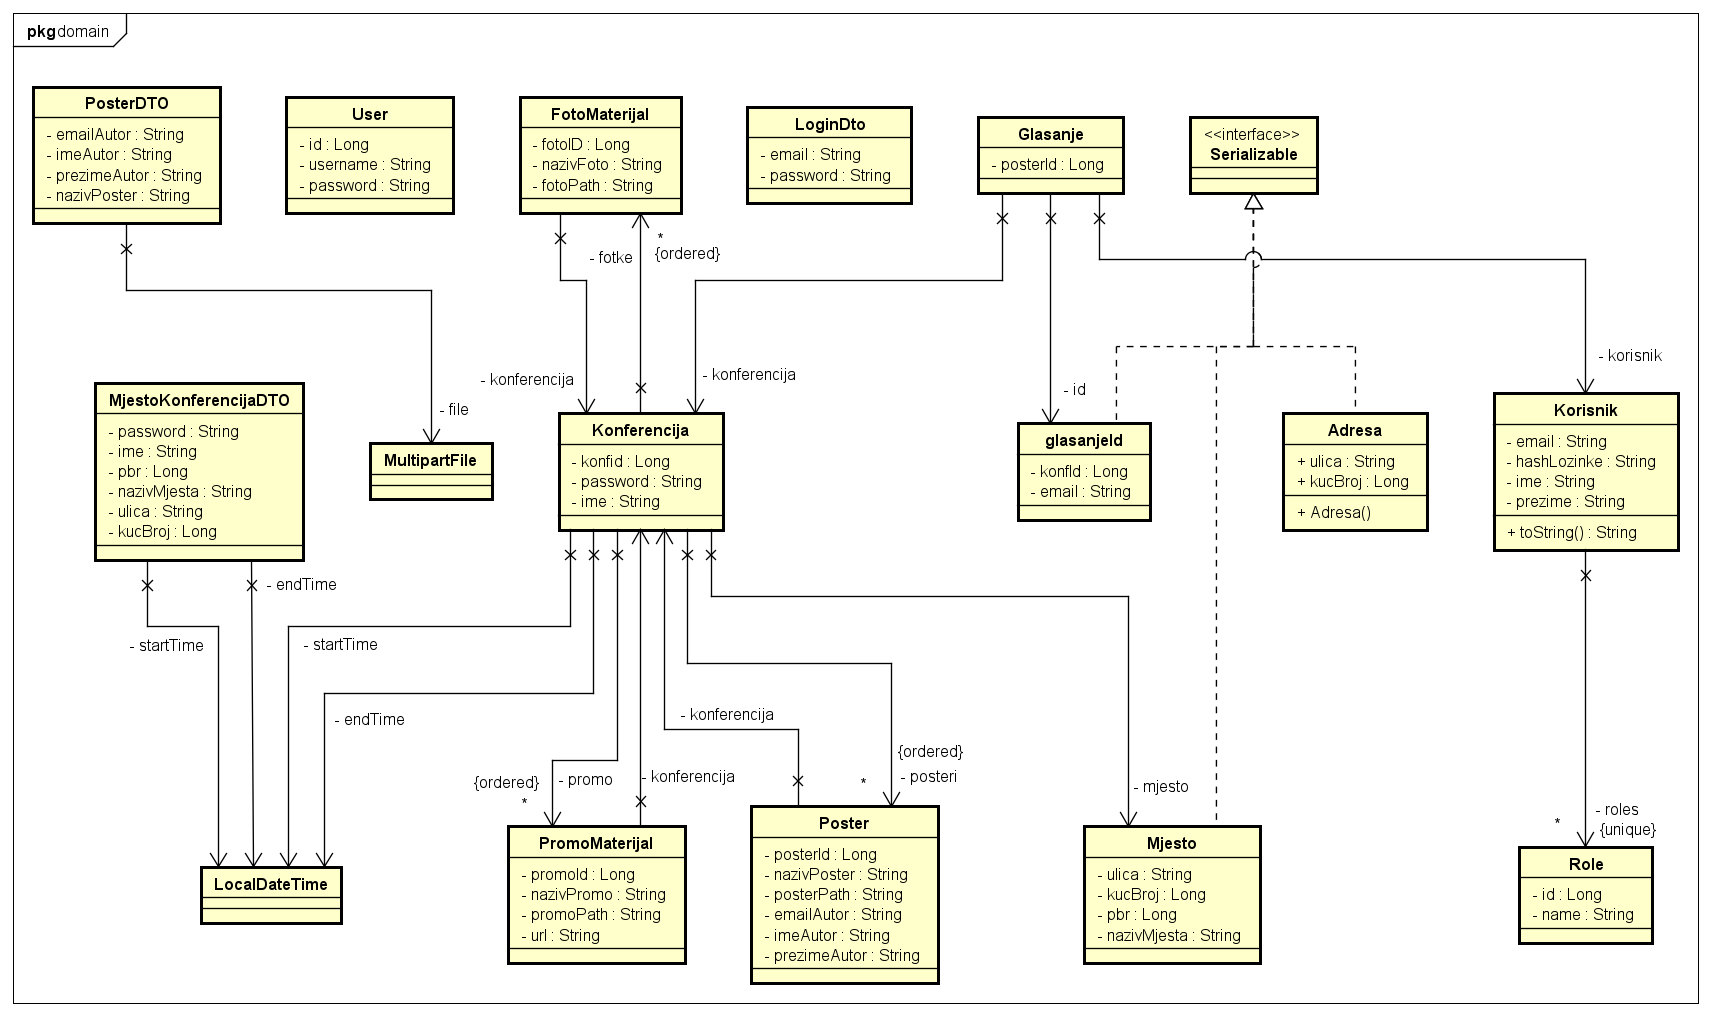
\includegraphics[width=\textwidth]{slike/domainClassDiagram.PNG} %veličina u odnosu na širinu linije
			\caption{Dijagram razreda - Domain}
			\label{fig:dr-domain} %label mora biti drugaciji za svaku sliku
		\end{figure}
		\newpage
		Sljedeći dijagram podijeljen je u 3 sloja: Controllers, Service i JPA koji sadrže pripadajuće razrede. Podjela je napravljena kako bi se postigla dobra organizacija i razdvajanje dijelova aplikacije. Sloj Controllers sadrži sve kontroler razrede te je njihova glavna uloga obrada HTTP zahtjeva. Sloj Service sadrži sučelja koja implementiraju razredi kontrolera. Oni pružaju apstrakciju između kontrolera i sloja podataka (JPA). Sloj Java Persistence API (JPA) zadužen je za pristup podacima u relacijskoj bazi podataka i za mapiranje java objekata u odgovarajući tip podatka u bazi podataka.
		\begin{figure}[H]
			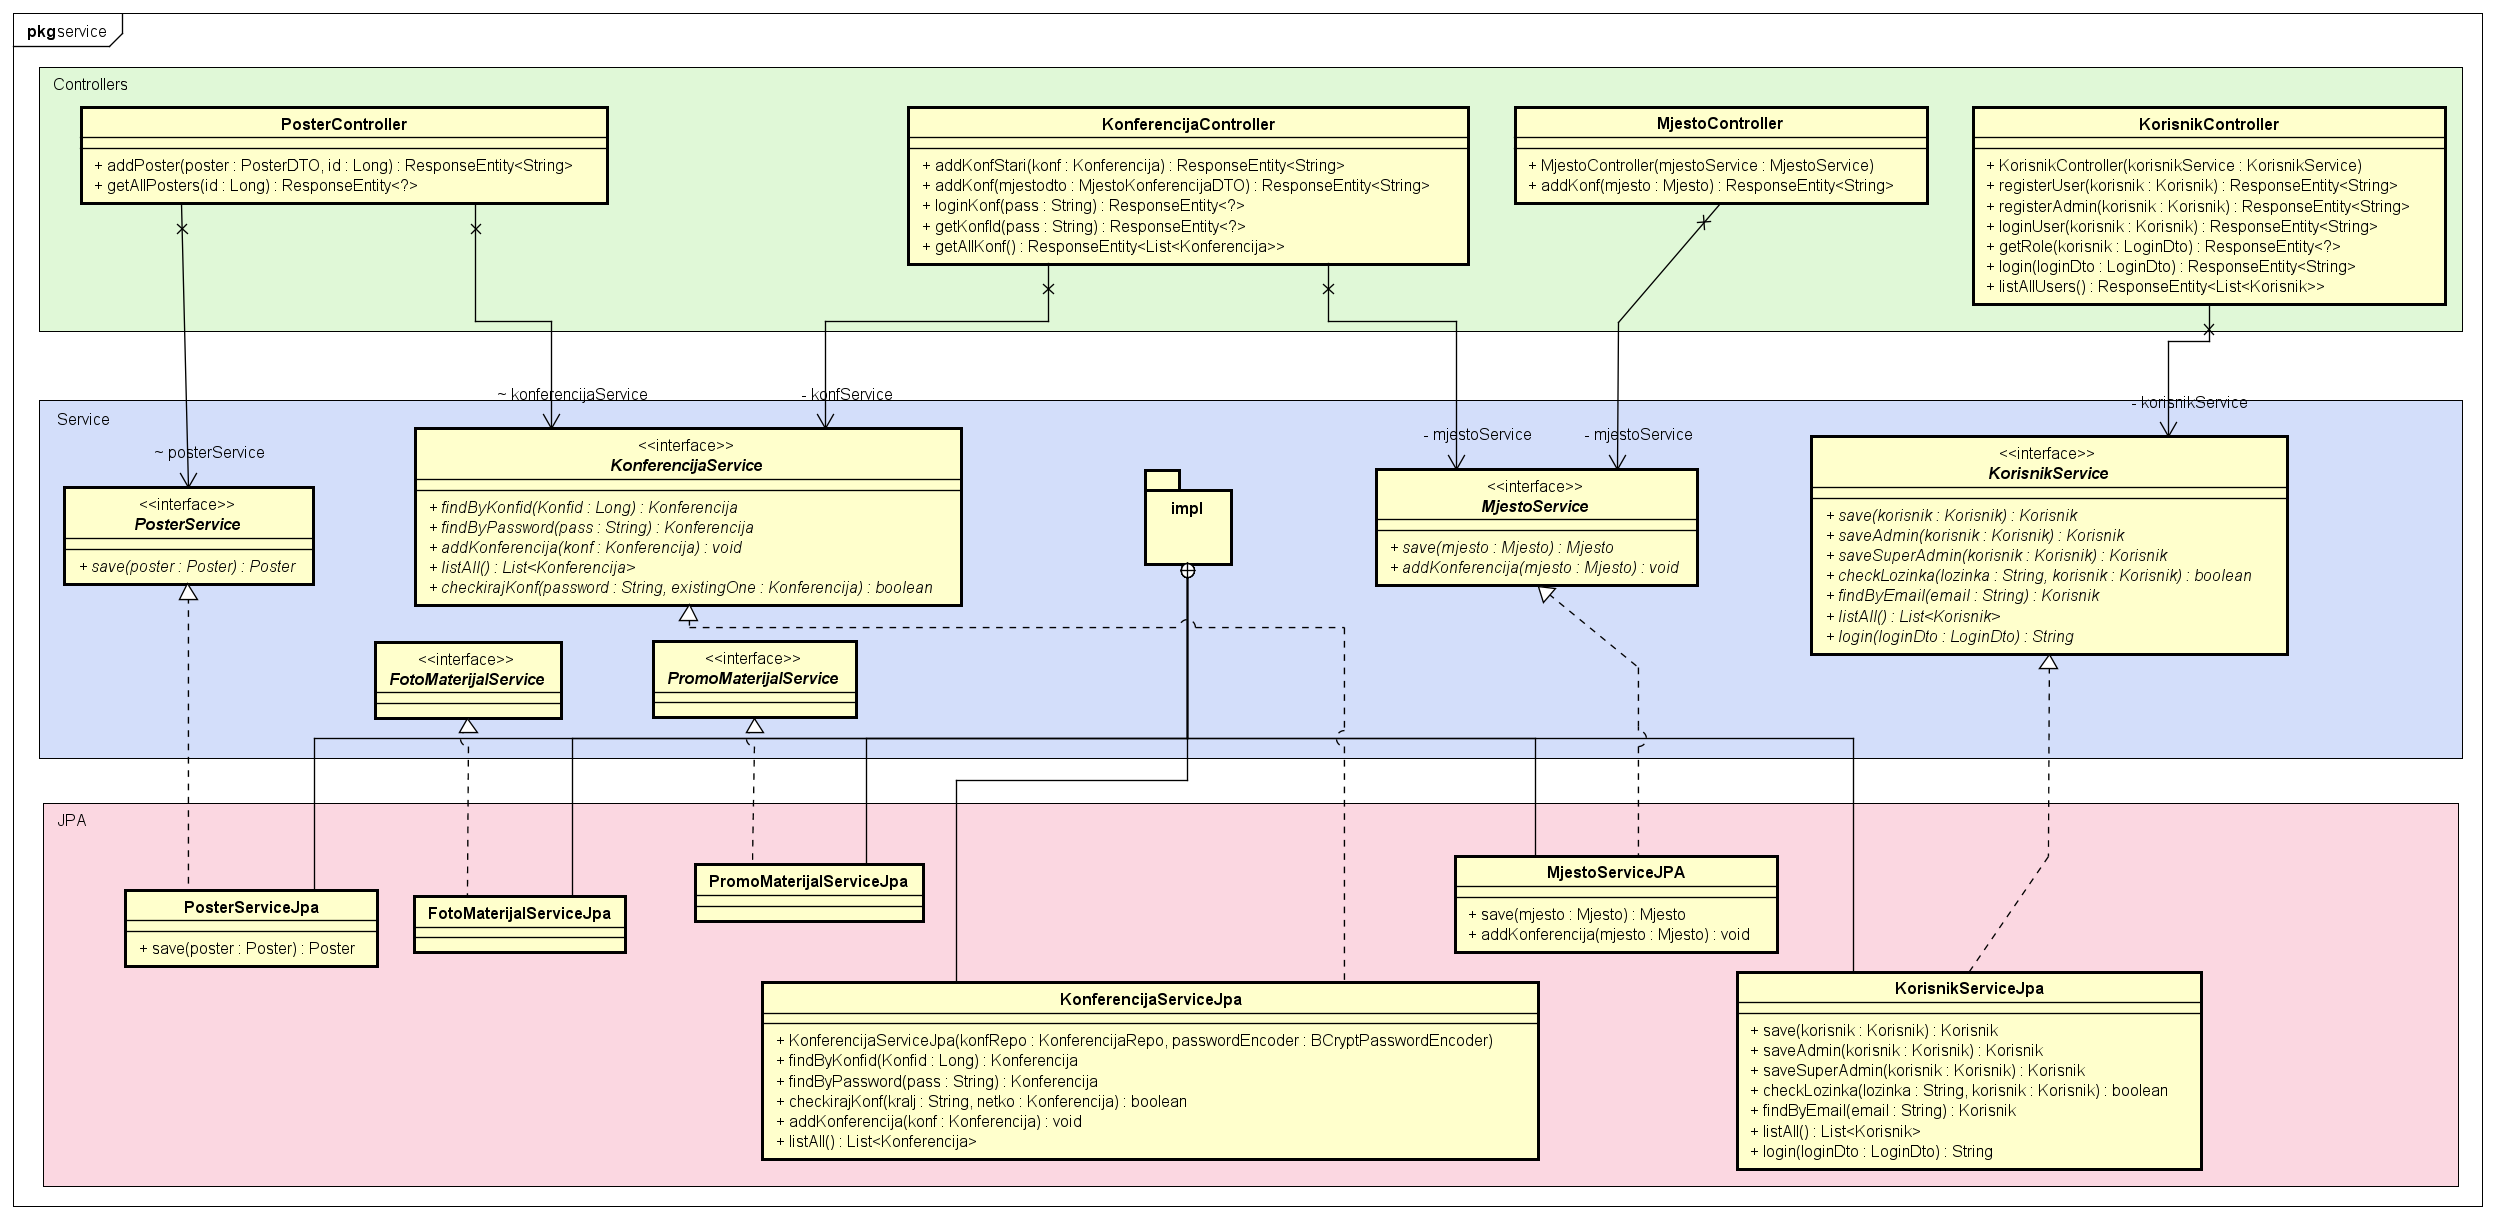
\includegraphics[width=\textwidth]{slike/serviceClassDiagram.PNG} %veličina u odnosu na širinu linije
			\caption{Dijagram razreda - Service}
			\label{fig:dr-service} %label mora biti drugaciji za svaku sliku
		\end{figure}
			\eject

		\section{Dijagram stanja}


			\textbf{\textit{dio 2. revizije}}\\

			\textit{Potrebno je priložiti dijagram stanja i opisati ga. Dovoljan je jedan dijagram stanja koji prikazuje \textbf{značajan dio funkcionalnosti} sustava. Na primjer, stanja korisničkog sučelja i tijek korištenja neke ključne funkcionalnosti jesu značajan dio sustava, a registracija i prijava nisu. }
			
			TODO opis
			
			\begin{figure}[H]
				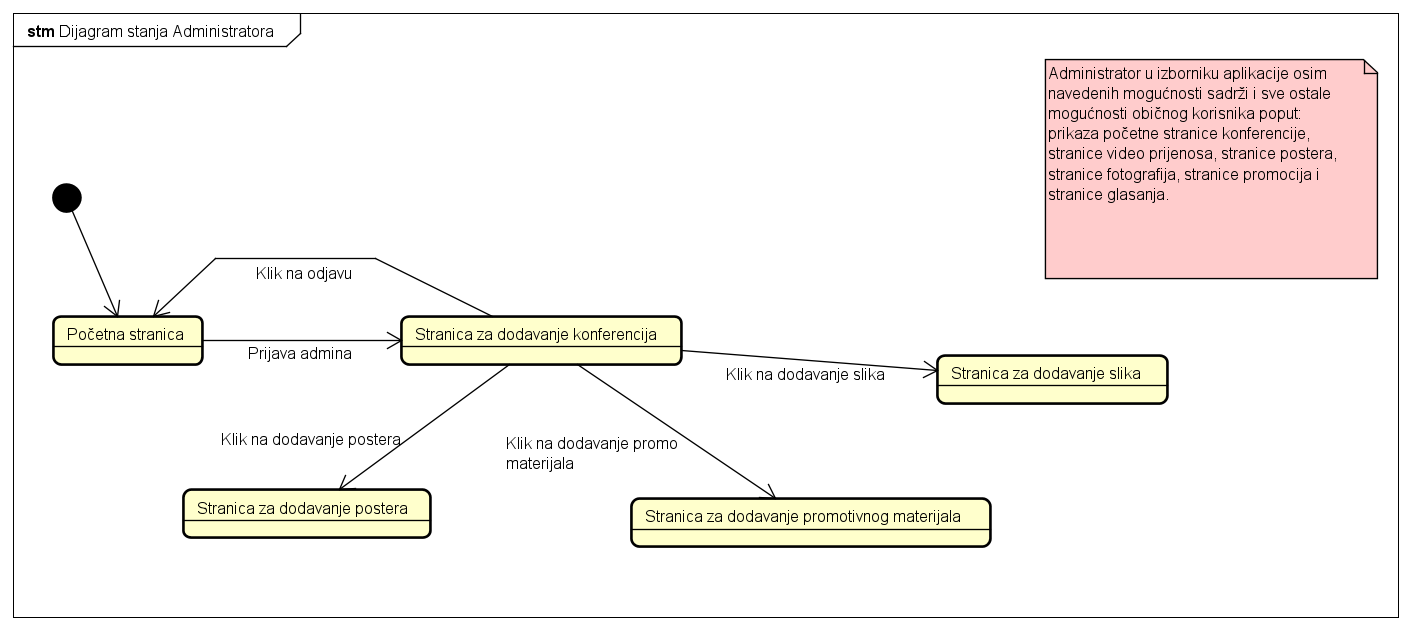
\includegraphics[width=\textwidth]{slike/adminStanja.PNG} %veličina u odnosu na širinu linije
				\caption{Dijagram stanja: mogućnosti administratora}
				\label{fig:adminStanje} %label mora biti drugaciji za svaku sliku
			\end{figure}
			\begin{figure}[H]
				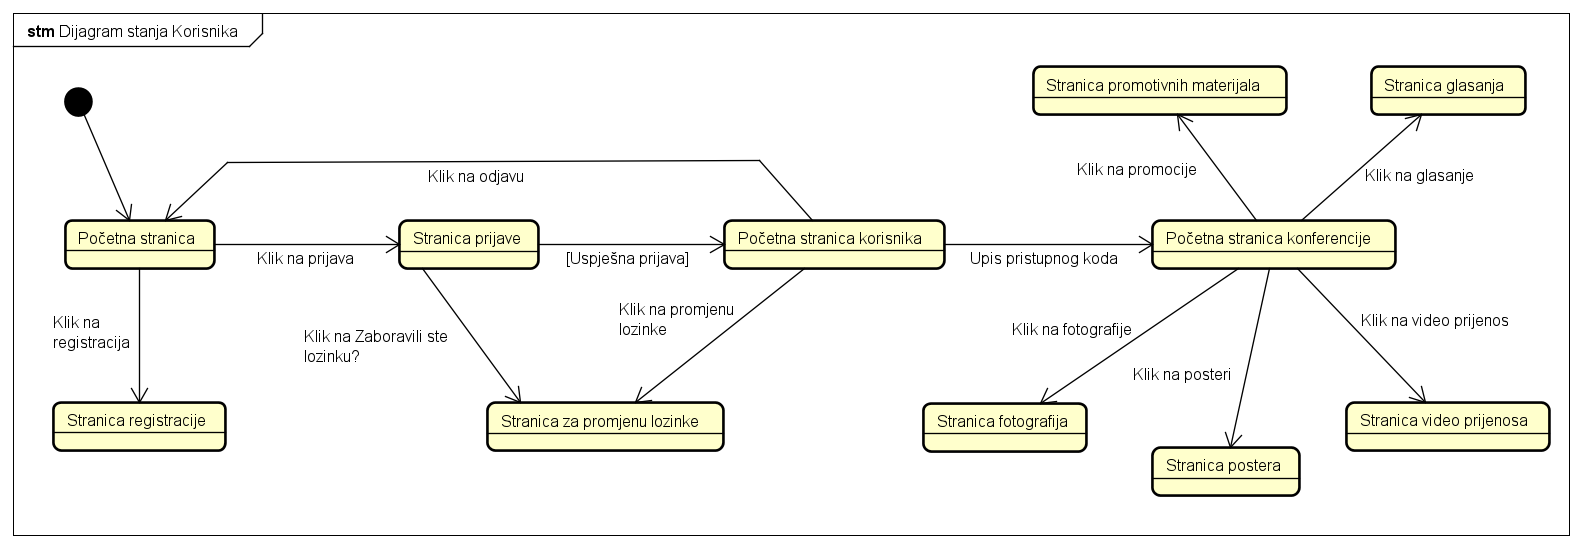
\includegraphics[width=\textwidth]{slike/korisnikStanja.PNG} %veličina u odnosu na širinu linije
				\caption{Dijagram stanja: mogućnosti korisnika}
				\label{fig:korisnikStanje} %label mora biti drugaciji za svaku sliku
			\end{figure}


			\eject

		\section{Dijagram aktivnosti}

			\textbf{\textit{dio 2. revizije}}\\

			 \textit{Potrebno je priložiti dijagram aktivnosti s pripadajućim opisom. Dijagram aktivnosti treba prikazivati značajan dio sustava.}
			
			TODO opis
			
			\begin{figure}[H]
				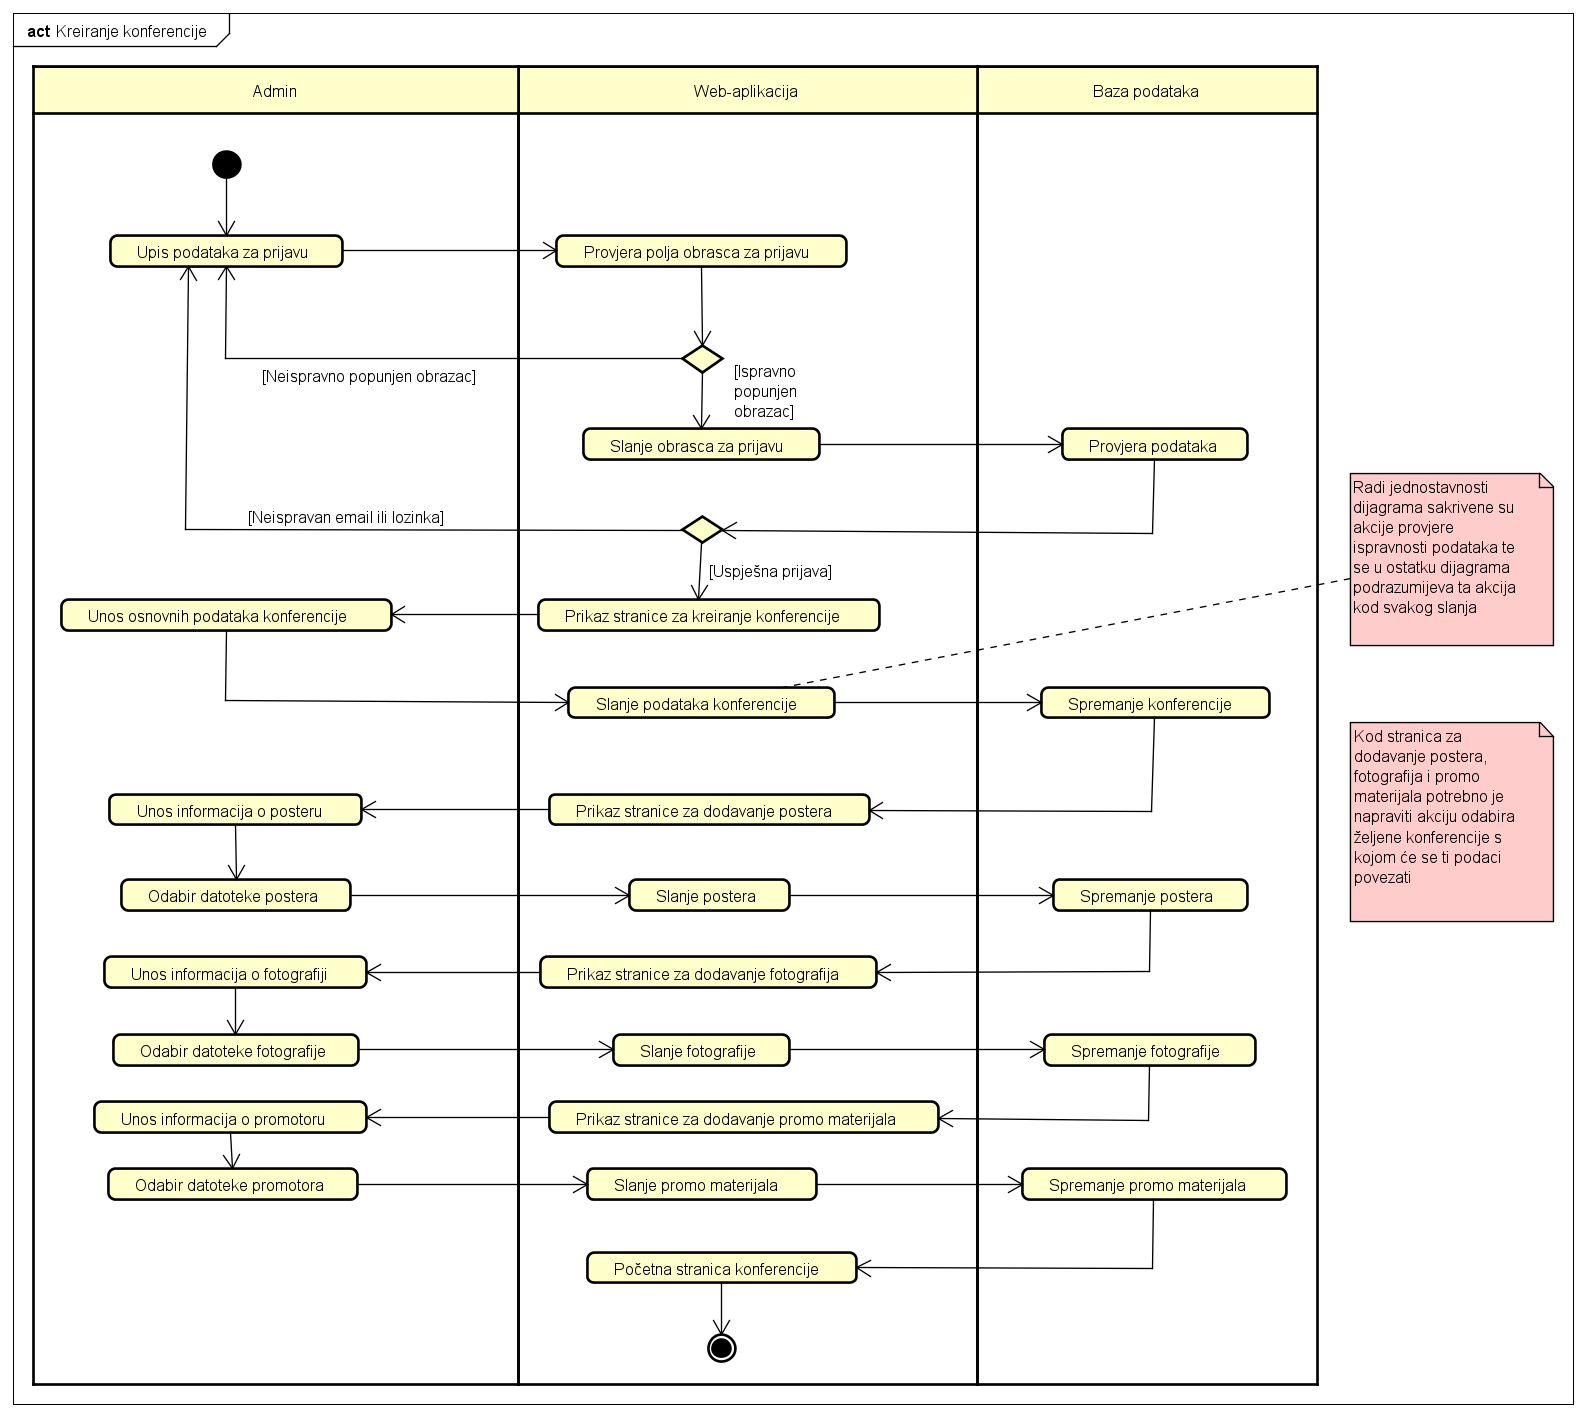
\includegraphics[width=\textwidth]{slike/dijagramAktivnosti.PNG} %veličina u odnosu na širinu linije
				\caption{Dijagram aktivnosti: kreiranje konferencije}
				\label{fig:dijagramAktivnosti} %label mora biti drugaciji za svaku sliku
			\end{figure}
			
			\eject
		\section{Dijagram komponenti}

			\textbf{\textit{dio 2. revizije}}\\

			 \textit{Potrebno je priložiti dijagram komponenti s pripadajućim opisom. Dijagram komponenti treba prikazivati strukturu cijele aplikacije.}
			 
			 TODO opis
			 
			 \begin{figure}[H]
			 	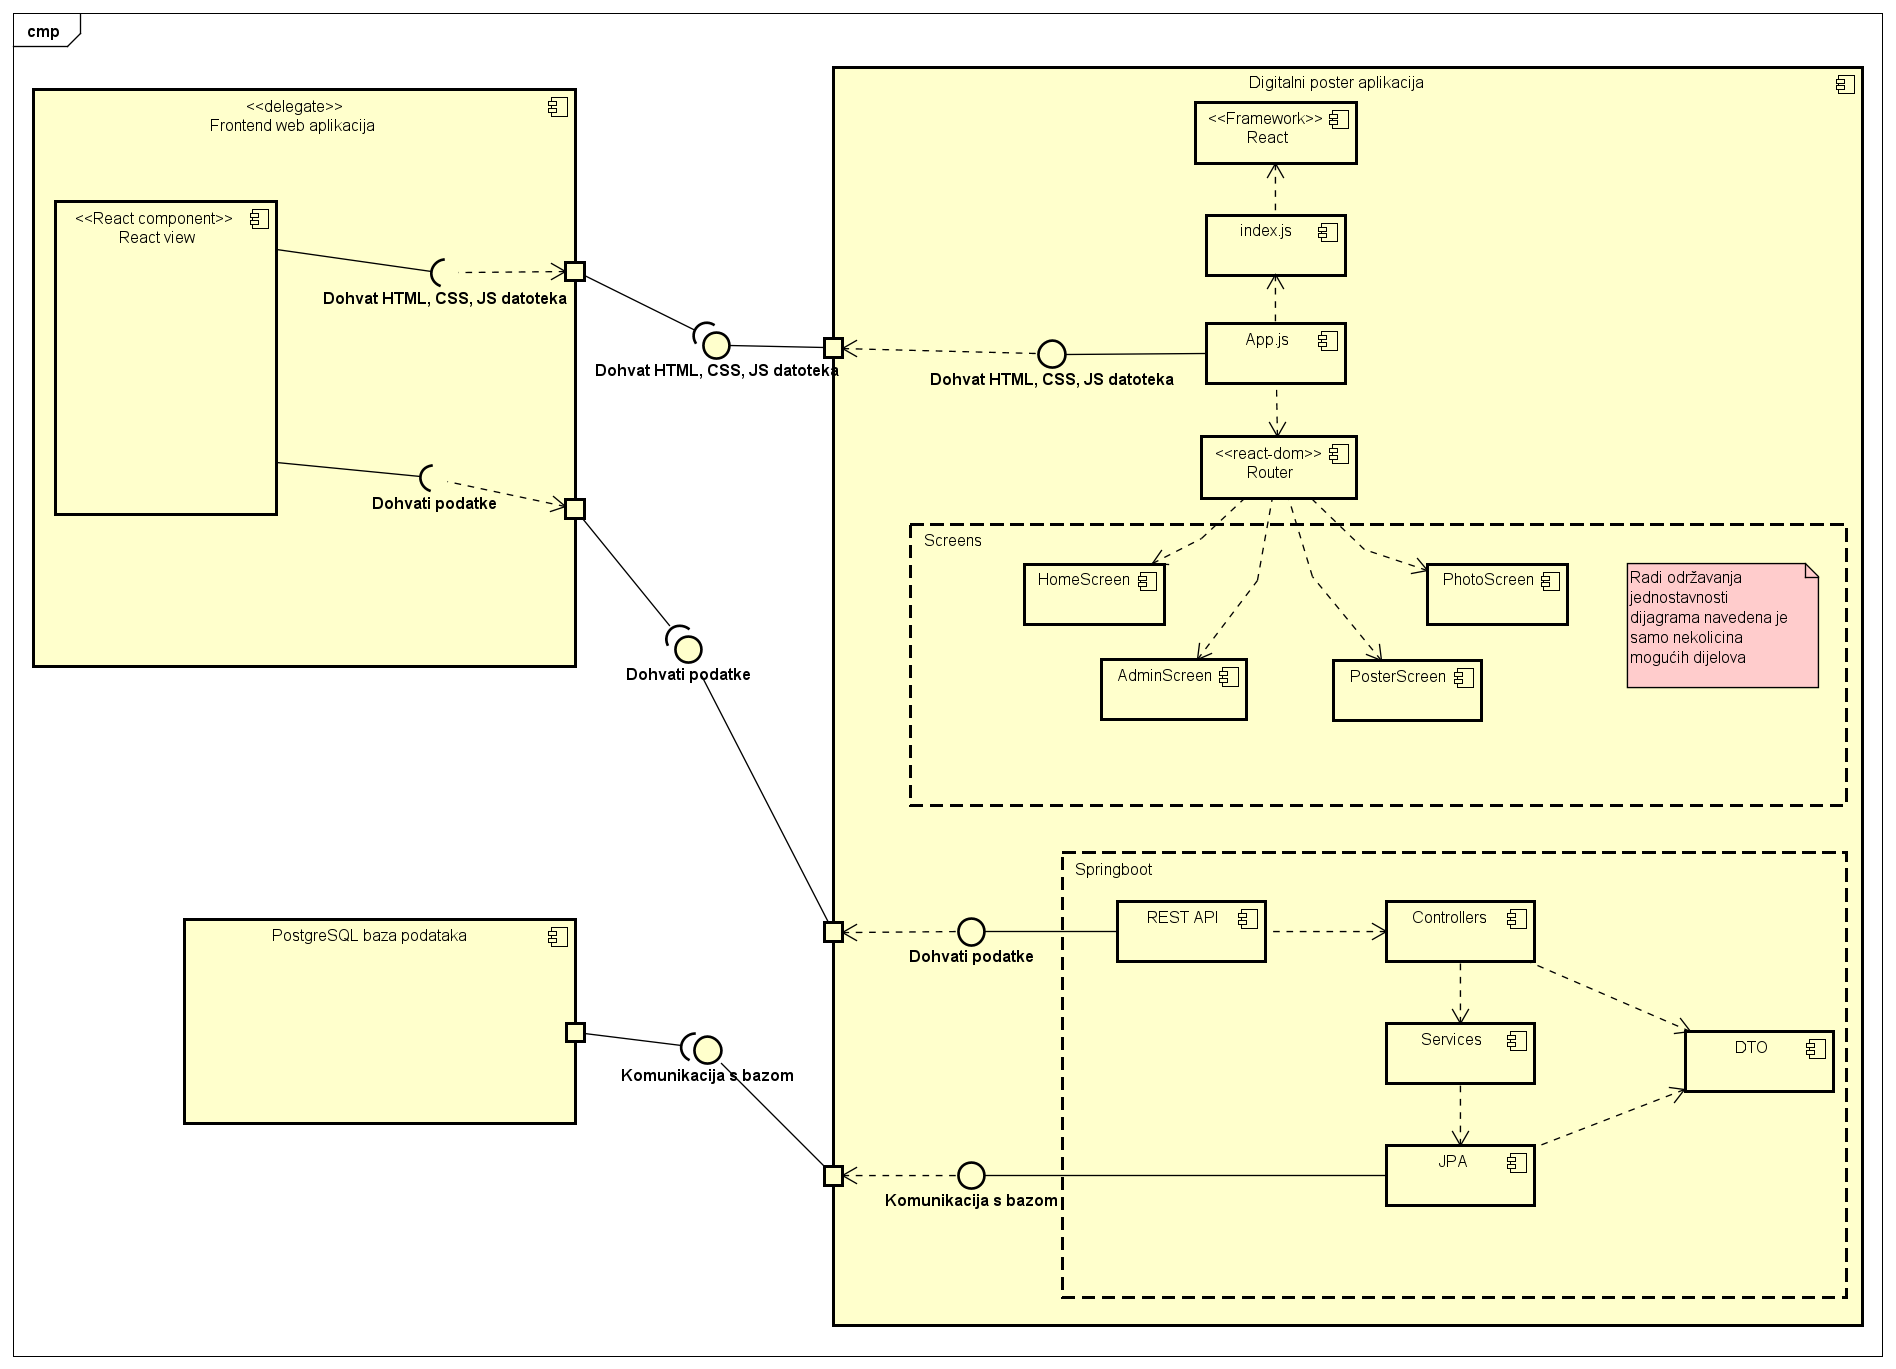
\includegraphics[width=\textwidth]{slike/dijagramKomponenti.PNG} %veličina u odnosu na širinu linije
			 	\caption{Dijagram komponenti}
			 	\label{fig:dijagramKomponenti} %label mora biti drugaciji za svaku sliku
			 \end{figure}
			 